\documentclass[a4paper,titlepage]{report}
\usepackage[T1]{fontenc} % codifica dei font
\usepackage[utf8]{inputenc} % lettere accentate da tastiera
\usepackage[italian]{babel} % lingua del documento
\usepackage{url} % per scrivere gli indirizzi Internet
\usepackage[sans,nouppercase]{frontespizio}

\begin{document}

\begin{frontespizio}
\Universita{Verona}
\Facolta{Informatica}
\Corso[Laurea]{Informatica}
\Titoletto{Tesi di laurea}
\Titolo{Internet of Things: un progetto di smart parking}
\Candidato{Aurora Bussola}
\Relatore{Prof. Nicola Fausto Spoto}
\Annoaccademico{2020-2021}
\Rientro{1.5cm}
\NCandidato{Laureando}
\Punteggiatura{}
\end{frontespizio}

\begin{abstract}
L'evoluzione digitale ha permesso ad Internet di espandersi coinvolgendo non solo computer networks ma pure diverse tipologie di dispositivi creando un legame fra il mondo virtuale e concreto. L'innovazione coinvolge un'infinità di ambiti, per questo motivo possiamo trovare dispositivi smart fra i più disparati: dalle macchinette del caffè connesse al WiFi di casa a dispositivi biomedicali come i pacemaker\cite{Ansari:BasedHealthcareApplications}. Tutto ciò trova ragione di esistere se si va ad analizzare la natura dell'uomo e del suo ambiente: siamo circondati da cose e più in particolare sopravviviamo grazie a delle cose ed è questo motivo per cui quest'ultime dovrebbero essere più importanti di qualsiasi idea e/o informazione\cite{Ashton: ThatInternetofThings'Thing}.\\La tesi, dopo una breve parte introduttiva, prenderà in esame un parcheggio intelligente per automobili trovando una possibile soluzione con l'ausilio di una piattaforma hardware per la prototipazione che sarà constantemente connessa ad Internet. Verranno descritti in particolare tutti gli aspetti e le scelte progettuali anche attraverso schemi concettuali, immagini e pseudocodici.
\end{abstract}

\tableofcontents

\chapter{Internet of Things}
\section{Definizione}
L'{\itshape Internet of Things}  abbrev. {\itshape IoT} (oppure {\itshape Internet delle Cose}, in italiano) può essere visto come un'estensione dell'Internet da noi conosciuto che aggiunge diverse tipologie di network e sensori. Esso incrementa l'ubiquità di Internet permettendo l'interconnessione di svariate tipologie di oggetti opportunamente configurati\cite{Feng:InternationJournalOfCommunicationSystems}.
\section{Una breve storia}
Il termine {\itshape Internet of Things} è stato coniato nel 1999 da Kevin Ashton, direttore dell'Auto-ID Centre\footnote{un'organizzazione no profit con sede presso il MIT} all'interno del quale venne inventata la tecnologia {\itshape RFID} (acronimo di {\itshape Radio-Frequency IDentification}). L'invenzione soppianta il vecchio sistema barcode semplificando la gestione di beni in svariati ambiti: nel 2000 LG pianifica lo sviluppo un frigorifero intelligente in grado di {\itshape capire} se un determinato prodotto fosse presente o meno; tre anni dopo la tecnologia RFID entra nel programma SAVI\footnote{acronimo di {\itshape Navy sexual Assault Victim Interventition}, per la difesa alle vittime di tale delitto} e all'interno della grande catena di supermercati Walmart; nel 2008 viene esteso l'uso del protocollo IP a network di oggetti e nel 2011 nasce la {\itshape IPSO Alliance}, un forum di portata globale che arruola diversi colossi industriali per lo sviluppo dell’{\itshape Internet of Things}\cite{Suresh:StateArtReviewIoTHistoryTechnologyFieldsDeployment}.

\chapter{La tecnologia RFID}
\section{Definizione e funzionamento}
La tecnologia RFID, citata in precedenza, permette la lettura e/o scrittura di informazioni rigurdanti svariate tipologie di oggetti. Grazie al suo costo relativamente ridotto e al suo enorme potenziale, la tecnologia RFID viene tutt'ora largamente adoperata in progetti IoT.\\Ogni sistema RFID è composto da tre elementi: il primo è un'etichetta elettronica (tag) che memorizza l'informazione, il secondo è un apparato che si interfaccia col tag (interrogatore\footnote{solitamente è uno scrittore o un lettore}) e il terzo è un dispositivo che gestisce il collegamento fra RFID e database per la gestione dell'informazione\cite{Sun:ApplicationRFIDTechnologyLogisticsInternetofThings}.
\begin{figure}[h]
\centering
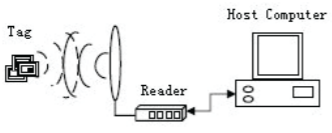
\includegraphics{schemaRFID.png}
\caption{Schema di funzionamento di un tipico sistema RFID}
\end{figure}
\section{La tecnologia RFID come valido sostituto al barcode}
Ci sono molti motivi per via dei quali la tecnologia RFID ha sostituito la più vecchia e obsoleta tecnologia barcode:
\begin{itemize}
\item Il tag non deve essere a contatto con l'interrogatore durante il trasferimento dell'informazione.
\item Il tag non deve necessariamente essere visibile per essere scritto/letto.
\item La lettura/scrittura del tag non richiede intervento umano, ne consegue che il costo per la manodopera diminuisce e l'errore umano viene minimizzato.
\item Il range di lettura/scrittura è più ampio rispetto a quello del barcode.
\item I tag possono essere riscritti/modificati e possono ospitare una maggiore quantità di dati.
\item E' più facile creare un codice univoco all'interno del tag.
\item I tag sono meno sensibili a condizioni avverse (polvere, danni fisici ecc.).
\item Più tag possono essere letti simultaneamente\cite{Kaur:RFIDTechnologyPrinciplesAdvantagesLimitationsApplications}.
\end{itemize}
\section{Applicazione in progetti IoT}
La tecnologia RFID non solo viene adoperata largamente in ambito commerciale, ma anche in altri ambiti non strettamente economici come in quello sanitario e militare. La ragione per la quale venga ancora utilizzata, nonostante abbia compiuto più di vent'anni, è data dal fatto che sappia constantemente adattarsi al cambiamento e alla costante evoluzione dell'IoT\cite{Xiaolin:RFIDTechnologyApplicationsIoT}.\\
\begin{figure}[h]
\centering
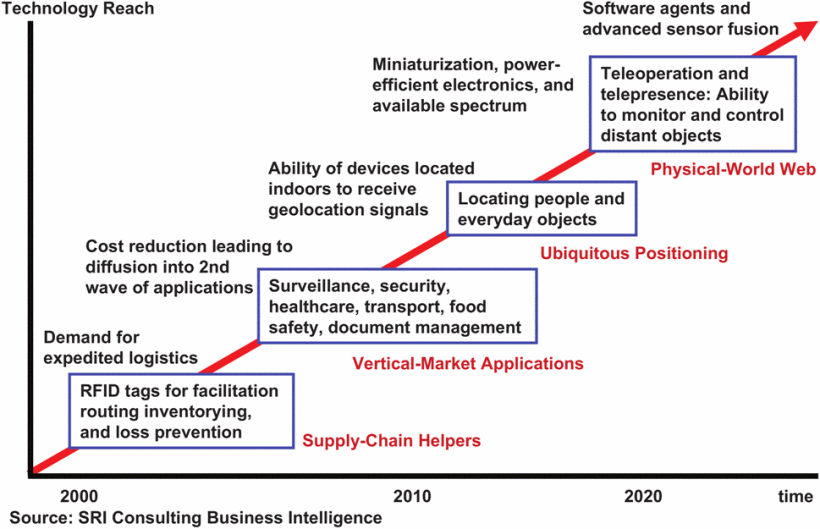
\includegraphics[scale = 0.3]{graficoRFID.png}
\caption{La tecnologia RFID si evolve con l'evolversi di IoT}
\end{figure}


% Bibliografia
\begin{thebibliography}{99}
\bibitem{Ansari:BasedHealthcareApplications}
Seema Ansari, Tahniyat Aslam, Javier Poncela, Pablo Otero, Adeel Ansari,
\emph{introduzione di Internet of Things-Based Healthcare Applications},
\url{https://www.igi-global.com/chapter/internet-of-things-based-healthcare-applications/243907}.
\bibitem{Ashton: ThatInternetofThings'Thing}
Kevin Ashton,
\emph{That 'Internet of Things' Thing},
\url{http://www.itrco.jp/libraries/RFIDjournal-That%20Internet%20of%20Things%20Thing.pdf}.
\bibitem{Feng:InternationJournalOfCommunicationSystems}
Feng Xia, Laurence T. Yang, Lizhe Wang, Alexey Vinel,
\emph{Internation Journal Of Communication Systems.}
\bibitem{Suresh:StateArtReviewIoTHistoryTechnologyFieldsDeployment}
P. Suresh, J. Vijay Daniel, V. Parthasarathy, R. H. Aswathy,
\emph{A state of the art review on the Internet of Things (IoT) history, technology and fields of deployment}
\url{https://ieeexplore.ieee.org/abstract/document/7043637}.
\bibitem{Sun:ApplicationRFIDTechnologyLogisticsInternetofThings}
Chunling Sun,
\emph{Application of RFID Technology for Logistics on Internet of Things}
\url{https://www.sciencedirect.com/science/article/pii/S2212671612000200}.
\bibitem{Kaur:RFIDTechnologyPrinciplesAdvantagesLimitationsApplications}
Mandeep Kaur, Manjeet Sandhu, Neeraj Mohan, Parvinder S. Sandhu,
\emph{RFID Technology Principles, Advantages, Limitations And Its Applications}
\url{http://ijcee.org/papers/306-E794.pdf}
\bibitem{Xiaolin:RFIDTechnologyApplicationsIoT}
Xiaolin Jia, Quanyuan Feng, Taihua Fan, Quanshui Lei,
\emph{RFID technology and its applications in Internet of Things (IoT)}
\url{https://ieeexplore.ieee.org/abstract/document/6201508}
\end{thebibliography}

\end{document}

